\section{Теоретическое введение}
В работе изучаются поперечные колебания стальной гитарной струны, натянутой горизонтально и закрепленной между двумя неподвижными зажимами. Так как поперечные размеры струны много меньше её длины, то напряжение в струне может быть направлено только \textit{вдоль неё}. В натянутой струне возникает \textit{поперечная упругость}, то есть способность сопротивляться всякому изменению формы, происходящему без изменения объёма. При вертикальном смещении произвольного элемента струны, возникают силы, действующие на соседние элементы, и в результате вся струна приходит в движение в вертикальной плоскости, т.е. возбуждение «бежит» по струне. Передача возбуждения представляет собой \textit{поперечные бегущие волны}, распространяющиеся с некоторой скоростью в обе стороны от места возбуждения. В ненатянутом состоянии струна не обладает свойством поперечной упругости, и поперечные волны на ней невозможны.

\subsection{Уравнение волны на струне}
Рассмотрим гибкую однородную струну, в которой создано натяжение T, и получим дифференциальное уравнение, описывающее её малые
поперечные свободные колебания. Отметим, что, если струна расположена
горизонтально в поле тяжести, величина T должна быть достаточна для
того, чтобы в состоянии равновесия струна не провисала, т.е. сила натяжения должна существенно превышать вес струны.
\noindent
Направим ось $x$ вдоль струны в положении равновесия. Форму волны будем описывать функцией $y(x,t)$, определяющей вертикальное смещение $y$ струны в данной точке в любой момент времени $t$. Рассмотрим малый элемент $dm$ струны. Так как амплитуда колебаний невелика, то можно пренебречь добавочным напряжением, возникающим из-за удлинения элементов струны и считать силу $T$ натяжения нити постоянной по её длине. Также можно считать углы отклонения $\alpha$ струны от оси $x$ малыми. В итоге по 2 закону Ньютона в проекциях на ось $y$ для элемента получим:
\begin{figure}
\center{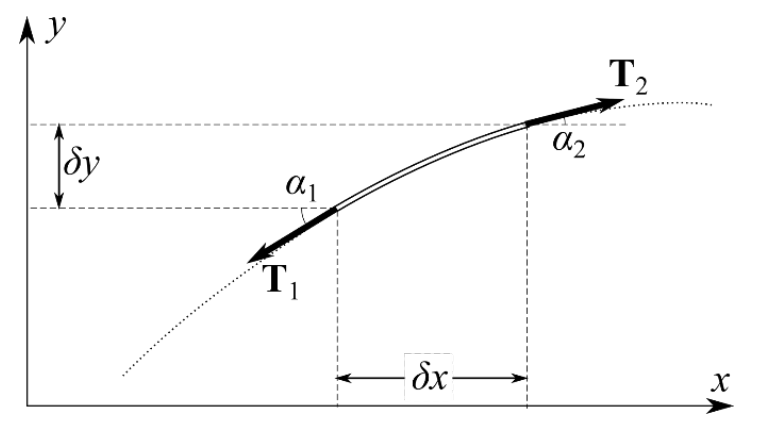
\includegraphics[scale=0.9]{image1.png}}
\caption{. \textit{К выводу уравнения колебаний струны}}
\end{figure}
\begin{equation}
T \alpha_2 - T \alpha_1 \approx \frac{\partial^2 y}{\partial t^2} dm
\end{equation}
Учтём, что в ненатянутом положении длина элемента равна $\delta x$, то есть $dm = \rho \delta x$, где $\rho$ - линейная плотность нити в ненатянутом состоянии. Тогда, учитывая, что $\alpha = \partial y/\partial x$, получим:
\begin{equation}
T\delta \alpha = \frac{\partial^2 y}{\partial t^2} \rho \delta x \Rightarrow \frac{\partial^2 y}{\partial t^2} = \frac{T}{\rho} \frac{\partial^2 y}{\partial x^2} = u^2 \frac{\partial^2 y}{\partial x^2} \quad \left(u = \sqrt{\frac{T}{\rho}}\right)
\end{equation} 
\fbox{%
\begin{minipage}{0.3 \linewidth} 
\centering
$\frac{\partial^2 y}{\partial t^2} = u^2 \frac{\partial^2 y}{\partial x^2} \quad (*) $
\end{minipage}}
- \textit{уравнение свободных малых поперечных колебаний в струне}. Оно также называется волновым уравнением.

\subsection{Бегущие волны}
Заметим, что произвольная функция вида $y(x,t) = f(x-ut)$ является решением волнового уравнения $(*)$. Действительно, обозначим $\psi(x,t) = x-ut$. Тогда 
\begin{equation}
y(x, t) = f(\psi(x,t)) \Rightarrow \frac{\partial y}{\partial t} = \frac{df}{d\psi} \frac{\partial \psi}{\partial t} \Rightarrow \frac{\partial^2 y}{\partial t^2} = \frac{\partial \psi}{\partial t} \left(\frac{d^2 f}{d\psi^2} \frac{\partial \psi}{\partial t}  \right) + \frac{df}{d\psi} \frac{\partial^2 \psi}{\partial t^2}
\end{equation}
Аналогично:
\begin{equation}
\frac{\partial^2 y}{\partial x^2} = \frac{\partial \psi}{\partial x} \left(\frac{d^2 f}{d\psi^2} \frac{\partial \psi}{\partial x}  \right) + \frac{df}{d\psi} \frac{\partial^2 \psi}{\partial x^2}
\end{equation}
\begin{flalign*}
\text{Учитывая, что } \ \frac{\partial \psi}{\partial t} = u, \ \frac{\partial^2 \psi}{\partial t^2} = 0, \ \frac{\partial \psi}{\partial x} = 1 , \ \frac{\partial^2 \psi}{\partial x^2} = 0 \text{, получим:} &&
\end{flalign*}
\begin{equation}
\frac{\partial^2 y}{\partial t^2} = u^2 \frac{d^2 f}{d\psi^2} = u^2 \frac{\partial^2 y}{\partial x^2}
\end{equation}

\noindent
Заметим теперь, что если в уравнении $y(x, t) = f(\psi(x,t))$ положить $\psi = const$, то получим: $dx/dt = u$, то есть возмущение струны движется поступательно со скоростью $u$ вдоль оси $x$.

\noindent
Общее же решение волнового уравнения представимо в виде суперпозиции двух волн произвольной формы, бегущих вдоль оси $x$ со скоростями $\pm u$:
\begin{equation}
y(x,t) = f_1(x-ut) + f_2(x+ut)
\end{equation}
Вид функций $f_1$ и $f_2$ в данной конкретной задаче определяется из начальных и граничных условий.
В данной работе будут изучаться \textit{гармонические волны}:
\begin{equation*}
y(x,t) = a \cos\left[k(x - ut)\right] + b \cos\left[k(x+ut)\right] = 
\end{equation*}
\begin{equation}
= a\cos\left(\omega t - kx\right) + b\cos\left(\omega t + kx\right)
\end{equation}
Здесь $\omega$ - циклическая частота колебаний, а $k = \frac{\omega}{u} = \frac{2\pi}{\lambda}$ - \textit{пространственная частота} волны. ($\lambda$ - длина волны).

\subsection{Собственные колебания струны. Стоячие волны} 

\noindent
Найдем вид свободных колебаний струны с \textit{закрепленными концами}. Пусть струна закреплена в точках $x = 0$ и $x = L$. Тогда из условия $y(0, t) = 0 \ (\forall t)$, получим:
\begin{equation}
a \cos(\omega t) + b \cos(\omega t) = 0 \Rightarrow a = -b
\end{equation} 
Тогда:
\begin{equation}\label{eq9}
y(x,t) = a(\cos(\omega t - k x) - \cos(\omega t + k x)) = 2 a \sin{kx} \cdot \sin{\omega t}
\end{equation}

\noindent
Нетрудно видеть, что данная волна получается в результате суперпозиции двух гармонических бегущих навстречу друг другу волн с равными амплитудами. Такая волна называется \textit{стоячей}. Вся струна колеблется с циклической частотой $\omega$. При этом амплитуда колебаний распределена по струне по закону: $y_m(x) = 2 a \sin{kx}$. В точках, где $\sin{kx} = 1$, амплитуда колебаний максимальна (\textit{пучности волны}). Точки, у которых $\sin{kx} = 0$ не колеблются вовсе (\textit{узлы волны}). Точки струны между двумя соседними узлами всегда колеблются в одной фазе, то есть в любой момент времени их скорости сонаправлены.

\noindent
Используем второе граничное условие $y(L, t) = 0 \ (\forall t)$:
\begin{equation}
\sin{kL} = 0 \Rightarrow kL = \pi n, \quad n \in \mathbb {N} 
\end{equation}
Тогда:
\begin{equation}
\lambda_n = \frac{2L}{n}, \quad n \in \mathbb{N}
\end{equation}
Как видно, параметр $n$ определяет число полуволн (то есть пучностей), которые умещаются на струне. Так как длина волны однозначно связана с её частотой, то струна может колебаться только с определёнными частотами:
\begin{equation}\label{eq12}
\nu_n = \frac{u}{2L} n
\end{equation}
Спектр собственных частот $\nu_n$ колебаний струны зависит только от её натяжения, линейной плотности и длины и, в случае малых гармонических колебаний, не зависит от модуля Юнга материала струны.

\subsection{Возбуждение колебаний струны. Резонанс} При колебаниях реальной струны всегда имеет место потеря энергии. Поддержание незатухающих
колебаний в струне может осуществляться точечным источником, в качестве которого в данной работе используется электромагнитный вибратор. 
Для эффективной раскачки колебаний используется явление резонанса - необходимо, чтобы вынуждающая частота $\nu$ вибратора совпала с одной из собственных частот $\nu_n$ струны. Тогда в любой момент времени потери энергии будут компенсироваться поступающей от воздбудителя колебаний энергией, процесс становится стационарным и можно наблюдать стоячие волны.

\noindent
Также стоит отметить, что в идеальном случае поток энергии вдоль стоячей волны отсутствует (в каждом участке между узлами кинетическая энергия переходит в потенциальную и наоборот). Однако, энергия от вибратора должна каким-то образом доходить до удалённых от него частей струны, поэтому в реальности помимо стоячей волны, есть ещё и малая бегущая компонента, которая и переносит энергию источника. Если потери энергии за период малы по сравнению с запасом колебательной энергии в струне, то искажение стоячих волн бегущей волной не существенно — наложение бегущей волны малой амплитуды на стоячую визуально приводит к незначительному «размытию» узлов (амплитуда колебаний в узлах совпадает с амплитудой бегущей компоненты волны).

\noindent
Для достижения максимальной раскачки колебаний, необходимо располагать возбуждающий контакт вблизи узловый точки (но не строго в ней). Действительно, предположим, что вибратор способен раскачать соответствующий элемент струны до амплитуды $A$. Если $x_0$ - расстояние от него до пучности, то из формулы \eqref{eq9}:
\[A = 2a \sin{kx_0} \Rightarrow a = \frac{A}{2\sin{kx_0}} \]
Отсюда видно, что расстояние $x_0$ следует устремлять к нулю.

\noindent
Наконец отметим, что в ходе работы необходимо добиться того, чтобы колебания были \textit{линейно поляризованы}, то есть чтобы струна колебалась в одной плоскости. Также необходимо обеспечить малость амплитуды колебаний - в противном случае волновое уравнение $(*)$ будет неприменимо.
